%TC:subst \shadow SHADOW
\section{Introduction}


\ac{mx} is a powerful tool for determining the three-dimensional structures of biological molecules at atomic resolutions \cite{Gorrec2021}. It has contributed significantly to our understanding of structure-function relationships in biology, protein folding, enzyme mechanisms, and structure-based drug-design \cite{Foerster2019}. Today, most of \ac{mx} is carried out at synchrotron beamlines due to the high brilliance and wavelength-tunability of synchrotron radiation, which are important features to crystallography experiments.

Beamline I23 at Diamond Light Source, the UK's national synchrotron, is a specialised synchrotron instrument operating at a wavelength range beyond that of standard \ac{mx} beamlines at 0.9-2.5 Å. While absorption is a minor effect in standard \ac{mx}, it becomes the largest source of error at increasingly long wavelengths. For this reason, I23 houses a tomography camera to analytically correct absorption coefficients from the sample in a diffraction experiment.
%Experiments are becoming more difficult and people are observing diminishing returns on their experimental data; this is met with efforts in developing more complex equipment. The demands for optimising the usage of these novel apparatuses directly drive the development of complex physical models. Coupled with the advent of powerful computers, the relevance of X-ray ray tracing simulations in designing better experimental equipment is evergrowing. The importance of which will only increase in light of new developments in free electron lasers and 4\textsuperscript{th} generation synchrotrons.


%In this section, the basic principles of synchrotron radiation are introduced, along with its applicability in the chemical sciences. An introduction to the pgm and the ray-tracing technique is discussed to highlight challenges of simulating pgm. This sets the stage for understanding specifically the challenge of higher harmonic contamination in soft X-ray beamlines and the detrimental effect it can have on the quality of the data. All of which serve to provide the motivation for developing more robust ray-tracing methodologies that would hopefully resolve potential issues in future beamlines from the outset. 
In this section, the basic principles of \ac{mx} phasing by anomalous diffraction are introduced, along with its applicability in long-wavelength crystallography at beamline I23. This sets the scene for understanding the challenges associated with long-wavelength crystallography and the need for more sophisticated absorption correction techniques to exploit the full potential of long-wavelength crystallography. % its full potential
All of this serves to provide the motivation for developing more robust, analytical absorption correction methods that would hopefully improve data quality and structure determination in future \ac{mx} experiments limited by high absorption.

%The data reduction techniques used to determine structure factor amplitudes and their uncertainties in \ac{xrd} are affected by factors like geometry, sample illumination, and X-ray absorption. 

% I23 uses novel approach of X-ray tomography coupled with a ray-tracing software for calculating absorption correction analytically. This paper discusses the findings of using an analytical approach to absorption corrections compared to standard empirical methods, as well as the combination of the methods. We go on to investigate whether this approach improves data in the ion identification experiments performed at I23.
%Furthermore, we investigate a second, more robust approach to absorption correction using laser-shaping to remove a majority of the non-diffracting material from the sample; this method is tested both empirically and analytically to determine whether there is a qualitative improvement in the combination of X-ray tomography-based segmentation and laser-shaping.

\subsection{Experimental Phasing in Macromolecular Crystallography}

%\ac{xrd} experiments provide the diffraction patterns of a crystal from the constructive interference of X-rays scattered by its electron clouds. Fourier methods are then implemented to calculate Fourier difference maps and to extract electron density maps from the diffraction spots. The resulting three-dimensional electron density $\rho$ for a given reflection $\hkl$, at position $(x,y,z)$ in a unit cell of volume $V$  can be expressed as: \cite{Taylor2003}

%\begin{equation}
    %\rho(x,y,z)=\frac{1}{V} \sum |F_{\hkl}| \exp(i\alpha_{\hkl}) \exp(-2\pi i [hx+ky+\ell z]) \label{electron_density}
%\end{equation}

%Where the atomic structure factor, $F_{hkl}$, is a measure of how efficiently each atom scatterers X-rays relative to an electron, given by:

In \ac{xrd} experiments, the diffraction patterns of a crystal are provided by constructive interference of X-rays scattered by the electron clouds. These patterns contain vital structural information about the crystal in the form of electron density maps, which can be extracted using Fourier methods. Our ability to solve for electron density, given by \cref{electron_density}, is hampered by the \textit{phase problem}, wherein the phases $\alpha_{\hkl}$ for a given reflection $\hkl$ are not directly solvable in experiment. 

%\begin{equation}
    %\mathbf{F}_{\hkl}= |F_{\hkl}| \exp{i \alpha_{\hkl}} = \sum_j f_j \exp{[2\pi i (hx_j + ky_j + lz_j]}
    %\label{structure_factor}
%\end{equation}

%And where $\alpha_{hkl}$ is the associated phase, $f_j$ is the scattering factor of atom \textit{j}, and $x_j, y_j, z_j$ are its positional coordinates.

%In \ac{xrd}, the intensities of reflections are proportional to the square of the structure factor amplitudes ($I_{\hkl} \propto |F_{\hkl}|^2$). The amplitudes are therefore directly measurable from reflection intensities, while the phase $\alpha_{\hkl}$ is lost in experiment \cite{Taylor2003}.
%This results in the\textit{ phase problem} as there is no unique solution to \cref{electron_density} without knowing $\alpha_{hkl}$. %Phases therefore carry important structural information that is necessary for producing accurate electron density maps.

\begin{equation}
    \rho(x,y,z)=\frac{1}{V} \sum |F_{\hkl}| \exp(i\alpha_{\hkl}) \exp(-2\pi i [hx+ky+\ell z]) \label{electron_density}
\end{equation}
% prop to square root of refkection intensity
%a measure of how efficiently each atom scatterers X-rays relative to an electron
\cref{electron_density} illustrates how electron density is proportional to the amplitude of the atomic structure factor, $F_{hkl}$, a measure of the scattering power for reflection $\hkl$. Here, $x,y,z$ are the positional coordinates of reflection $\hkl$ in a unit cell of volume $V$, where $\hkl$ are the Miller indices describing the orientation of the crystal plane in reciprocal space. %by quantifying its reciprocal intercepts in the crystal axes.

Experimental phasing is concerned with solving the phase problem to extract structural information from diffraction experiments. One set of techniques which have become the preferred phasing methods in \ac{mx} rely on anomalous scattering, a phenomenon observed in the X-ray absorption of matter.

Anomalous scattering occurs when an incident X-ray has a wavelength close to an element’s absorption edge, leading to the photon being absorbed instead of scattered. A possible outcome of anomalous scattering is fluorescence, when higher energy electrons drop to lower energy shells. The more common outcome, most relevant to the present case, is the immediate re-emission of radiation, resulting in an imaginary phase shift. This causes the overall atomic scattering factor $f$ to experience a change in amplitude, described by a real dispersive term $f’$, and a change in phase, described by an imaginary absorptive term $f”$:

\begin{equation}
    f=f^0+f'(\lambda)+if''(\lambda) \label{total scattering}
\end{equation}

This behaviour is element-specific and exhibits a strong dependence on the wavelength of the incident radiation, making the phenomenon particularly useful for element identification as well as phasing.

\begin{figure}
    \centering
    \input{./images/Normal and anomalous scattering.txt}
    \caption{(A) Normal scattering: Friedel's law is obeyed; (B) Breakdown of Friedel's law in the presence of an anomalous scatterer; the amplitudes of reflections are given by $F_P$ for the native crystal and $F_{PH}$ for the derivative. The isomorphous difference, $F_H \approx F_{PH} - F_P$, is an estimate of the heavy-atom structure. Adapted from Taylor, G. \cite{Taylor2003}.}
    \label{Breakdown of Friedel's law}
\end{figure}
% add side-by-side picture of Friedel's law obeyed
% replace labels with f = f0 + f' + if"

Experimental phasing by anomalous diffraction takes advantage of the differences in amplitude between Friedel pairs to determine the phase angles. In \ac{mad}, phases are determined using the orthogonal information from anomalous dispersion recorded at multiple wavelengths. \Ac{sad}, on the other hand, requires phase ambiguity resolution either in the form of a structural derivative labelled with an anomalous scatterer, a common example being methionine labelled with selenium to form selenomethionine, or by using the anomalous signal of natively present atoms in what is known as native \ac{sad}.

Native \ac{sad} is considered an attractive phasing technique in  \textit{de novo} X-ray structure determination %in MX,
for exploiting weak signals from intrinsic anomalous scatterers \cite{Basu2019}, with its most popular applications being on native sulphur and phosphorous \cite{Karasawa2022}. However, native \ac{sad} has its challenges in \ac{mx}, largely owing to the fact that standard beamlines are optimised around the Se K-edge at 12.7 \unit{keV} (0.979 Å) to allow for experiments on selenomethionine (\ce{C5H11NO2Se}) and Se-incorporated proteins.
While the absorption edges relevant to metalloproteins therefore typically lie in the accessible wavelength range of most standard \ac{mx} beamlines (0.9-2.5 Å), %(5-12 \unit{keV})
several light atoms native to nucleic acids and proteins (including sulphur and phosphorous), have absorption edges beyond the reach of most current \ac{mx} beamlines (5.02 Å and 5.78 Å respectively) \cite{Olieric2016}. 

%thus
Native \ac{sad} is in turn typically performed at 'compromise' energies of around 6 \unit{keV}, which is far from the absorption edges of the aforementioned light atoms. The resulting anomalous signal is small and systematic errors from radiation damage need to be minimised to accurately measure reflection intensities \cite{DjinovicCarugo2005}.%(Djinovic-Carugo, 2005). %This renders many biologically useful native SAD experiments inaccessible to most MX beamlines. 

%hindered by the necessity to access longer X-ray wavelengths
%in order to make most use of the anomalous scattering contributions of these elements. Presented here are the results from a first successful experimental phasing study of a macromolecular crystal structure
%at a wavelength close to the sulfur K edge. This has been made possible by the in-vacuum setup and the long-wavelength optimised experimental setup at the I23 beamline at Diamond Light Source. In these early commissioning experiments only standard data collection and processing procedures have been applied, in particular no dedicated absorption correction has been used.

Data collection at energies lower than 6 \unit{keV} is attractive for the native \ac{sad} phasing of macromolecules for this reason \cite{Omari2023}. This is demonstrated %corroborated
by beamline I23 at Diamond Light Source, arguably one of the most specialised \ac{mx} beamline in the world \cite{Foerster2019}. %In addition to phasing, another use of anomalous diffraction is for ion identification, which is another primary focus of beamline I23.%epitomised

\subsection{Beamline I23: Long-wavelength Macromolecular Crystallography}

Diamond Light Source (DLS) is a third generation, medium energy synchrotron based in the United Kingdom. It houses 32 beamlines, each using synchrotron radiation in different scientific and engineering disciplines and applications, including protein structure, materials science, and engineering innovations.
I23 is a unique long-wavelength \ac{mx} beamline capable of operating at wavelengths between 1.1 and 5.9 Å \cite{Wagner2016}.

The wavelength range at I23 covers the absorption edges of
%several anomalous scatterers of biological importance, such as sulphur, potassium, chlorine, and phosphorous. 
light elements often present in macromolecules (P, S, Cl, K, Ca, Mg).
Native \ac{sad} experiments performed at I23 enable phasing without the need for additional labelling by exploiting the anomalous scattering from these atoms at sufficiently long wavelengths. Some of the first succesful native \ac{sad} experiments at I23, at a wavelength close to the sulphur K-edge, demonstrated both the necessity for accessing longer wavelengths and that the capability to extract phase information can be even further improved once data collection and processing protocols have been optimised \cite{Aurelius2017}.
%the need for derivatives such as selenomethionine.

Data collection wavelengths can be tuned to closely above and below the absorption edges, also enabling identification of the element type and location; an example of this application in experiment is known as $f"$-refinement, a novel method of ion identification recently developed at I23. % anomalous scattering at I23.%where the experimentally determined $f"$ elucidates the atom type. %this is the primary application of anomalous scattering at I23. %Ion identification using anomlous scattering is therefore a large focus of I23.

\begin{figure}[h]
    \centering
    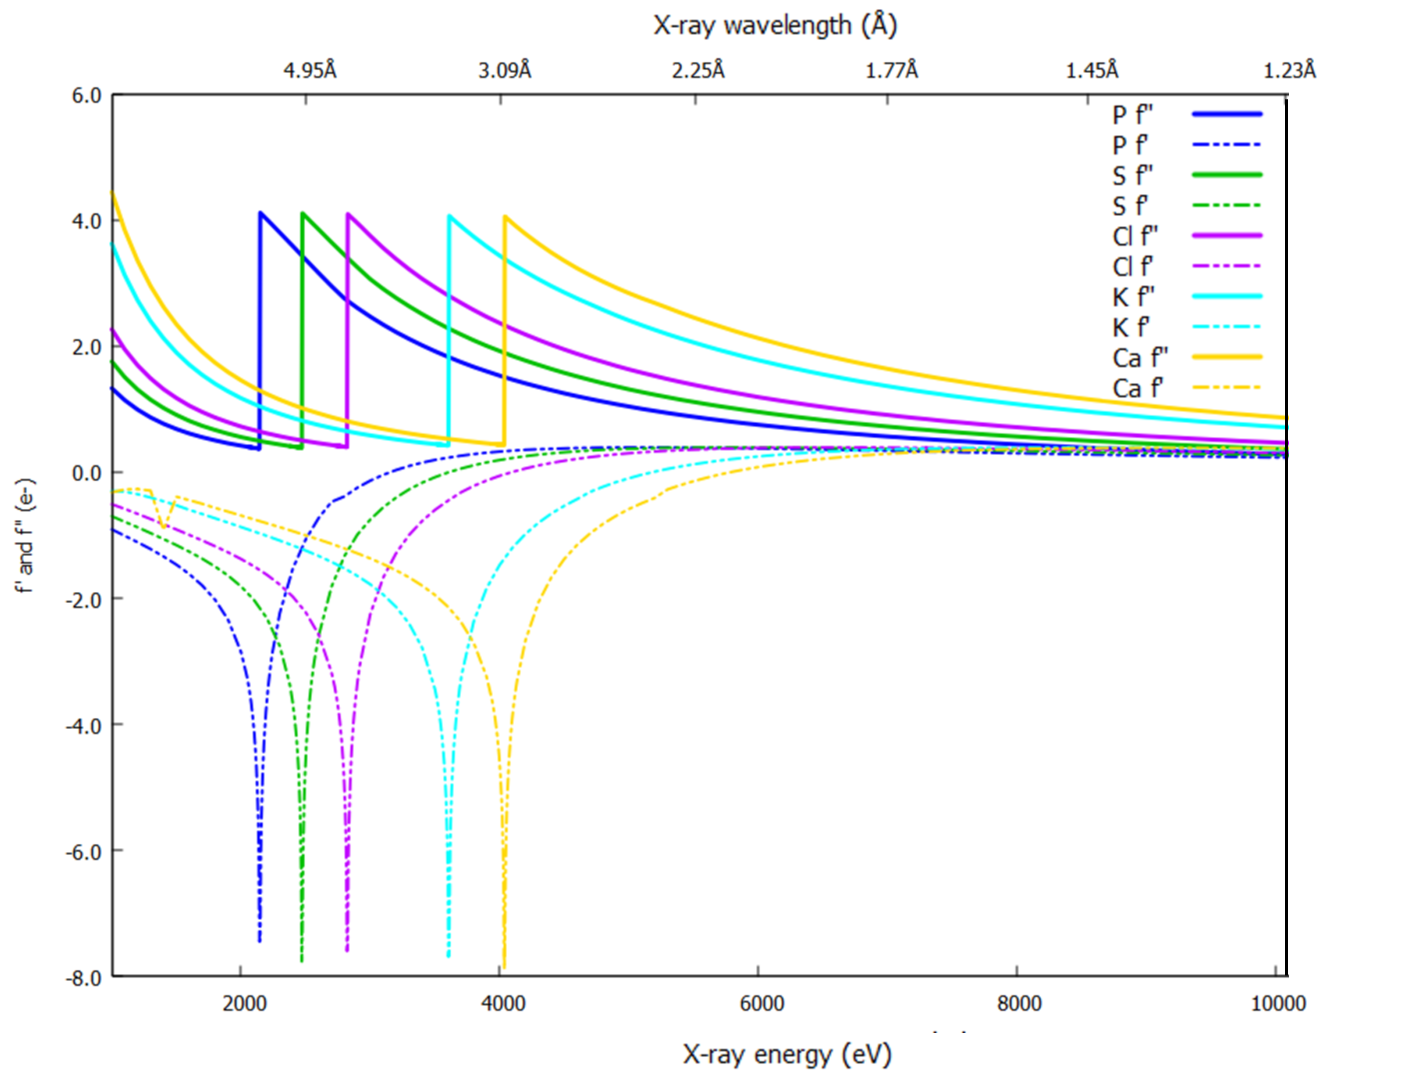
\includegraphics[width = 0.65\textwidth]{images/absorption lines high quality cropped.png}
    \caption{Characteristic X-ray lines of biologically relevant elements (P, S, Cl, K, Ca) accessible at I23 beamline energy range. Solid lines represent absorption ($f"$) edges and dashed lines represent dispersion ($f'$) edges. Adapted from the \href{http://skuld.bmsc.washington.edu/scatter/AS_periodic.html}{X-ray Absorption Edges} platform using the subroutine library by Brennan and Cowan \cite{Brennan1992}.}%anomalous scatterers common in macromolecules (P, S, Cl, K, Ca), showing the real dispersive term $f'$ and imaginary absorptive term $f''$. NB elements of a lower atomic number have emission lines at longer wavelengths. Produced by Brennan and Cowan. \cite{Brennan1992} }%NB the emission wavelength is critically affected by the molecular environment, and therefore unique to every atom in a structure.}
    \label{Anomaluos scattering edges}
\end{figure}

The need for the beamline's specialised operation stems from the complex challenges of operating at such low energies, which greatly reduce the quality of diffraction experiments.
%Low-energy \ac{xrd} is hindered by 
One source of hindrance is Bragg’s law, $nλ = 2d \sin(\theta)$, which states that the diffraction angle increases with wavelength. The highest resolution X-rays can therefore go unrecorded if they pass beyond the reach of the detector. The solution to this on I23 is a semi-cylindrical detector, the Pilatus 12M shown in \cref{fig:gonio_and_detector} (right), which allows most of the data to be detected. Nevertheless, data resolution is still limited by the detector’s geometry at the longest wavelengths.

 Another challenge is that sample absorption is approximately proportional to the cube of the wavelength, $\mu \propto \lambda^3$ \cite{Arndt1984}, making it a crucial limiting factor at long-wavelengths. The effects not only contribute to radiation damage, but also attenuate the diffracted X-rays within the sample \cite{Wagner2016}.

To eliminate the absorption of low-energy X-rays by gases, experiments are performed in-vacuum at temperatures below 100 K. This setup requires a dedicated endstation for the transfer of frozen samples from air to a vacuum environment. By operating in-vacuum at cryogenic temperatures, I23 eliminates air absorption and scattering while reducing radiation damage, increasing the signal-to-noise ratio even at the lowest energies.

\begin{figure}
    \centering
    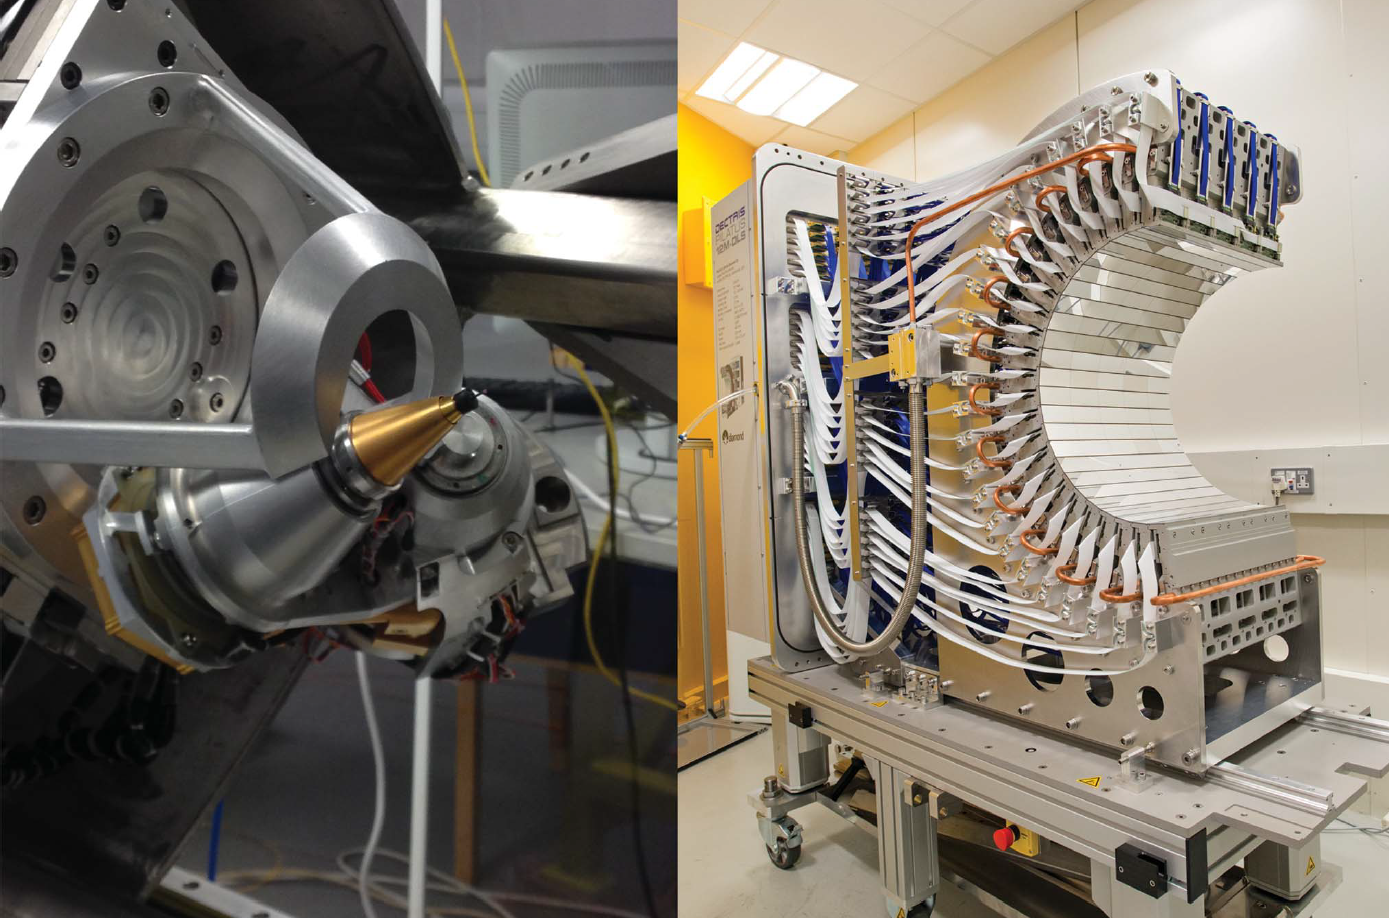
\includegraphics[width = 0.7\textwidth]{images/goniometer&detector.PNG}
    \caption{The kappa goniometer of the I23 endstation (left) and the Pilatus 12M before installation (right). Produced by Wagner \textit{et al.} \cite{Wagner2016}.}
    \label{fig:gonio_and_detector}
\end{figure}

% pictures of endstation + vacuum chamber + detector + crystream

Despite the specialised endstation at I23, the effects of absorption on experiments are still drastic at the longest wavelengths, and a correction is needed in response \cite{Kazantsev2021}.

\subsection{Absorption Correction Techniques at I23}

%The data reduction techniques used to determine structure factor amplitudes and their uncertainties in \ac{xrd} are affected by factors like geometry, sample illumination, and X-ray absorption. While the latter is a minor effect in standard MX, absorption becomes the largest source of error at increasingly long wavelengths.

%Away from absorption edges, the absorption of a sample is approximately proportional to the cube of the wavelength, $\mu \propto \lambda^3$ \cite{Arndt1984}. \ac{xrd} at long-wavelengths is therefore hindered by high absorption effects, such as X-ray scattering by air and low diffraction intensities. I23 mitigates some of these effects by operating in-vacuum, thereby increasing the overall signal-to-noise ratio.

%Another issue of low-energy MX stems from Bragg’s law, $nλ = 2d \sin(\theta)$, which states that the diffraction angle increases with wavelength. The highest resolution X-rays can therefore go unrecorded if they pass beyond the reach of the detector. The solution to this on I23 is a semi-cylindrical detector, Pilatus 12M, which allows most of the data to be detected. Nevertheless, data resolution is still limited by the detector’s geometry at the longest wavelengths.%, and several factors need to be considered to calculate structure factor amplitudes.

%Since high-quality structure determination relies on accurate structure factor amplitudes, 

Accounting for the absorption effects on Bragg’s intensities becomes critical at long wavelengths. For a lone crystal sample, the measured intensities corrected for absorption are given by $I_{corr} = I_{measured}/A_{\hkl}$, where the absorption correction factor, $A_{\hkl}$, for the reflection $\hkl$ is given by \cite{Albrecht1939}: %(Albrecht, 1939):

\begin{equation}
    A_{\hkl} = \frac{1}{V} \int_V \exp{-\mu(L_1+L_2)} dV
    \label{AbsFactor}
\end{equation}

Where $L_1$ and $L_2$ are the incident and diffracted X-ray paths for each crystal element $dV$ respectively, and $\mu$ is the X-ray absorption coefficient. \cite{Busing1957}

In a standard \ac{mx} experiment, X-rays transmit not only through the diffracting material but also the sample mount and surrounding solvent. This non-diffracting material is accounted for by expressing the absorption factor as:

\begin{equation}
    A_{\hkl} = \frac{1}{V} \sum_i \exp{-\mu_i (L_{1,i}+L_{2,i})} dV
    \label{AbsFactor_allmaterials}
\end{equation}

Where the sum is over $i$ materials exposed to the X-rays \cite{Santoro1968}. This analytical approach however requires precise information on the geometry of sample.

Absorption corrections are typically performed using empirical methods based on spherical harmonics \cite{Blessing1995}. \ac{sh} estimate the radii of spherical crystals to minimise differences between symmetry-related reflection intensities, with the first few models visualised in \cref{fig:SH}. %These models inherently assume a spherical shape of the diffracting material in question in data reduction.


\begin{figure}
    \centering
    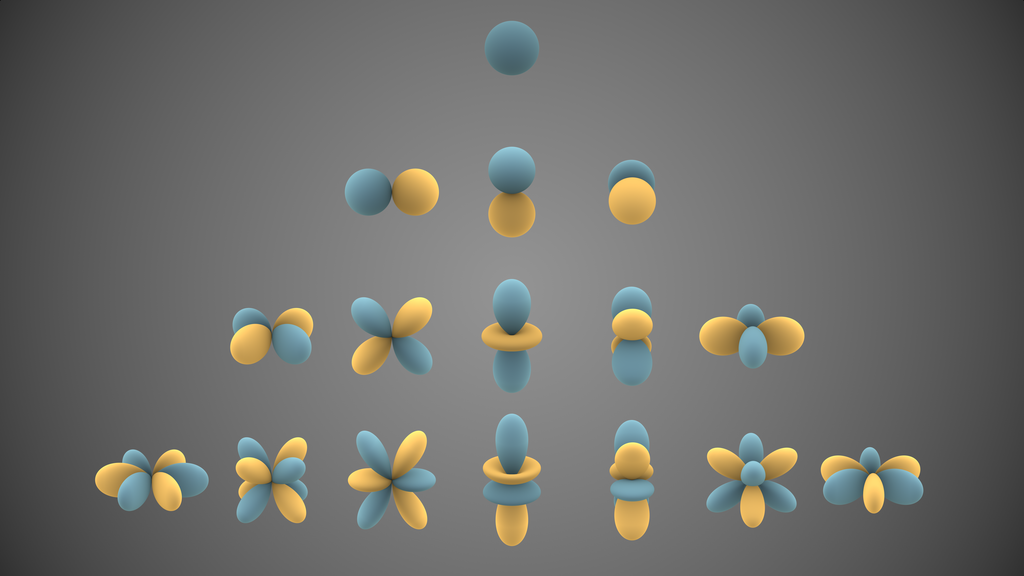
\includegraphics[trim={3cm 0 3cm 0},clip,width = 0.5\textwidth]{images/Spherical_Harmonics.png}
    \caption{Representation of the real component of the first few spherical harmonics models. Reproduced from Schönefeld (2005) \cite{Schoenefeld2005}.}
    \label{fig:SH}
\end{figure}

Most data reduction software in \ac{mx} use \ac{sh} as a basis for absorption correction calculations. This includes DIALS \cite{Winter2018}, the reduction software used as standard at Diamond Light Source.

Because empirical methods are independent of sample geometry, their efficiency depends on the number of symmetry equivalent reflections, which is limited by data multiplicity. Their applicability is therefore limited in low-symmetry space groups. More relevant to I23, empirical corrections become inadequate for modelling strong absorption effects above 3.5 Å, and an analytical correction is needed \cite{Kazantsev2021}.

%To analytically calculate the $A_{\hkl}$ factors in \cref{AbsFactor_allmaterials}, the shape and orientation have to be characterised in detail.
Characterising the shape and orientation in detail has previously been done using optical microscopy \cite{Leal2008, Strutz2011}. %(Leal 2008, Strutz 2011)
An alternative approach taken by I23 to obtain the 3D sample model is X-ray tomography, which has been applied previously to characterise and visualise crystals \cite{Merrifield2011, Warren2013}.%(Merrifield 2011, Warren 2013)

 It has previously been reported that using tomographic reconstructions and segmentation as a basis for absorption correction allows for the calculation of X-ray path lengths through all the different materials in the sample \cite{Brockhauser2008}. This tomography-based approach to corrections is the focus of this project.

By operating a tomography camera integrated into the endstation, I23 applies \ac{ac} based on a physical model of the sample derived from X-ray tomography, while empirical ones based on \ac{sh} are performed in the post-refinement step. Most relevant to this project is an approach that combines these two methods, by applying an empirical correction to the reconstructed physical model of the sample. This method is referred to as an \ac{acsh} in the remainder of this work. %in this project

This project will investigate tomographic reconstructions as a basis for calculating absorption factors with the help of \textbf{AnACor}, a novel ray-tracing software that has been developed collaboratively between I23, Graeme Winter at Diamond Light Source, and Yishun Lu at the Department of Engineering, University of Oxford. AnACor implements ray-tracing to estimate the path lengths of incident and diffracted X-rays through the sample \cite{Lu2024}, as illustrated in \cref{fig:analytical correction model}.

\begin{figure}
    \centering
    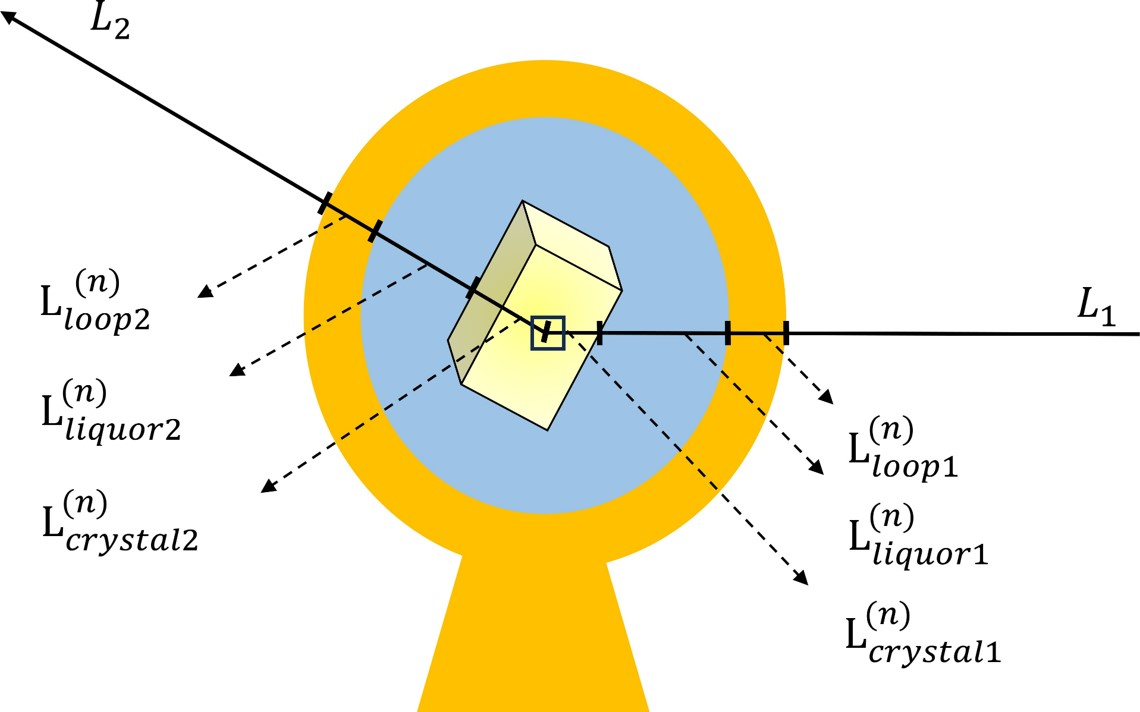
\includegraphics[width = 0.6\textwidth]{images/absorption correction diagram.jpg}
    \caption{Sketch illustrating the ray-tracing of absolute path lengths of X-rays through a sample, serving as the basis for analytically calculating absorption coefficients. $L_{m1}^{(n)}$ and $L_{m2}^{(n)}$ represent the path lengths of the incident and diffracted beams respectively for a material $m$. Adapted by Lu \textit{et al.} \cite{Lu2024}.
    % Fig. 1. A sketch illustrating the ray-tracing method used to calculate an absorption correction factor for a crystal voxel n. L(n)_m1 and L(n)_m2 represent the path lengths of m1	m2 the incident and diffracted X-ray beams through the material m (loop, liquor and crystal).
    }
    \label{fig:analytical correction model}
\end{figure}

AnACor calculates the absorption factors for materials in an analytical 3D model with a discrete form of \cref{AbsFactor}, where the integral over crystal elements $dV$ is replaced with a sum over the crystal voxels $\Delta V$ from  reconstruction \cite{Lu2024}: %applies an analytical absorption correction strategy based on the 3D model of the sample derived from X-ray tomography.

\begin{equation}
    A_{\hkl} = \frac{1}{N} \sum_{n=1}^N A_{\hkl}^{(n)}
\end{equation}

Where $N$ is the number of crystal voxels in the model exposed to the X-ray beam.

A second alternative correction technique, which is a newer but less established practice at I23, is laser-shaping. By operating a femtosecond laser optimised for cryo-crystallography samples, I23 can utilise laser-shaping to remove the non-diffracting material of a sample, leaving ideally only the diffracting material in a sample prior to the diffraction experiment. This thereby removes a significant amount of background noise, boosting the diffracting quality.

Previous studies have shown that both tomography-based reconstruction and laser-shaping can be beneficial for improving the detection of anomalous signal, but the effects of combining these practices has not yet been explored. This project sets out to do so by observing the data quality statistics of a laser-shaped crystal and a control from the same batch corrected with standard \ac{sh} practices, analytically (\ac{ac}), and with the coupled approach of the two (\ac{acsh}).

\subsection{Aims of the Project} %and Strategies

The main aims of this project are as follows:

\begin{enumerate}
    \item Establish the AnACor software produces valid experimental absorption coefficients from X-ray tomography
    \item Demonstrate the successes and shortcomings of tomography-based \ac{ac} and that of a coupled approach (\ac{acsh}) to standard practices (\ac{sh})
    %\item Test the ability of the analytical approaches in identifying sodium ions in lysozyme protein
    \item Assess the effects of tomography-based analytical corrections on $f"$-refinement
    \item Assess the effects of laser-shaping as an alternative absorption correction \textit{in-situ} and with tomography-based analytical corrections
\end{enumerate}